\documentclass[dvisvgm,tikz,border=4pt]{standalone}
\usepackage{amsmath,amssymb}

\usetikzlibrary{arrows.meta,positioning,automata,shapes,shapes.misc,calc,decorations.pathmorphing,decorations.markings,angles,quotes,patterns,mindmap,matrix,knots,hobby,trees}
\tikzset{->-/.style={decoration={markings, mark=at position 0.5 with {\arrow{Stealth}}}, postaction={decorate}}}
\begin{document}
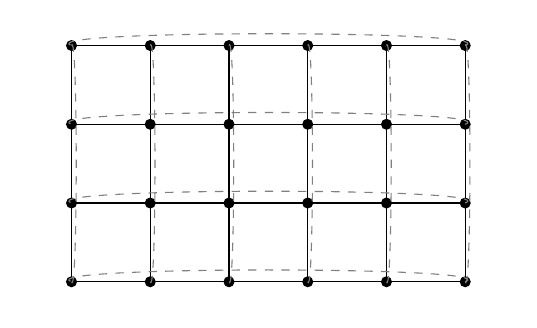
\begin{tikzpicture}
\foreach \x in {0,...,5} \foreach \y in {0,...,3} {
  \fill (\x,\y) circle (2pt);
  \ifnum\x<5 \draw (\x,\y) -- (\x+1,\y); \fi
  \ifnum\y<3 \draw (\x,\y) -- (\x,\y+1); \fi
}
\foreach \y in {0,...,3} \draw[dashed, gray] (5,\y) to[out=20, in=160, looseness=0.3] (0,\y);
\foreach \x in {0,...,5} \draw[dashed, gray] (\x,3) to[out=70, in=-70, looseness=0.2] (\x,0);
\end{tikzpicture}
\end{document}
